\chapter{相变的统计力学}\label{cha:相变的统计力学}

在前面的章节中,我们主要处理的是无相互作用粒子组成的系统。对于这类情况,只需知道系统各个组分的能级,就可以直接获悉整个系统的热力学函数。比热、平衡常数、能谱分布等都是隶属于这一类型的主要现象。我们发现这一类这些系统的热力学函数都有一个显著的特征——都是光滑连续的(除了玻色-爱因斯坦凝聚)。

但世界上还有另一类系统等待着统计力学,那就是 \textcolor{RoyalBlue}{\textbf{\kaishu 相互作用系统}}。对于这类情况,当我们研究系统的热力学函数时,会遇到解析上的不连续性和奇异性,并且粒子之间的相互作用再也无法通过坐标变换移除,以至于整个系统的能级与各单一组分的能级之间也就不再有简单的加和关系。在适当条件下,系统大量微观组分之间的相互作用还会变得非常强,从而各组分间呈现出 \textcolor{RoyalBlue}{\textbf{\kaishu 合作}} 行为。当系统的温度达到一个临界 $T_c$ 时,这样的合作行为还会具有宏观效应。

\begin{justification}{\kaishu 反思与质疑}
\kaishu \fontsize{11pt}{16pt}
    \quad\quad 光子气体的玻色-爱因斯坦凝聚的原因并不是相互作用,而是微观粒子的关联性。玻色子的交换对称性使得它们倾向于占据较为靠近的态,而费米子的交换反对称性使得它们倾向于占据较为远离的态(这里比较的对象是既不交换对称也不交换反对称的一般波函数)。这种关联性的结果可以等效为一个吸引势或者排斥势,但并不属于这里讨论的相互作用范畴。

    \quad\quad 另一个问题是:热力学函数是配分函数的偏导数,而配分函数求和的各项很明显是无穷阶可微的,怎么就奇异了呢?如果系统可及的微观态数量有限,那么导数算符的线性性和可微函数的加和性确实可以保证热力学函数处处连续可微,但问题在于有的时候求和的项是可数无限的,此时就会出现函数项级数的求导-求和什么时候可交换的问题,也就是配分函数的一致收敛问题。
\end{justification}

此外,这样的合作现象还具有一些本质的、不依赖于微观细节的特性。例如,系统的响应函数 $\chi $ 在临界点的奇异性,以及系统的各种热力学函数在临界点附近的非解析性。这些特性是相互作用系统的普遍特征,而不是某一特定系统的特征。这类系统的研究是统计力学的一个重要分支,称为 \textcolor{RoyalBlue}{\textbf{\kaishu 临界现象}} 的统计力学。

\textcolor{RoyalBlue}{\textbf{\kaishu 相变}} 集中体现着这些特点。为了简化因相互作用而导致的复杂问题,我们需要引入一些模型,这样的模型需要对相互作用做一定的简化,但仍然保留关于组分间合作行为的基本特性。至于模型能够将相互作用简化至何种程度,就取决于自然界所能呈现的最简单、最容易理解的相互作用是什么。

\textcolor{RoyalBlue}{\textbf{\kaishu 磁学系统}} 是一个比为理想气体添加中心势还要简单的模型——自旋只有一上一下两个状态,相邻自旋方向相同和相反将给出两个不同的相互作用能。如果将这些自旋磁子在一维、二维、三维空间中摆放整齐,并将各自旋之间除了最近邻相互作用能之外的项统统忽略,我们就将得到那个著名、普适、以及优雅的 \textcolor{RoyalBlue}{\textbf{\kaishu Ising 模型}}。


\section{磁学系统的热力学}\label{sec:磁学系统的热力学}

对于以往的理想气体、声子、光子系统,它们的热力学我们是见怪不怪的,也容易理解它们确实具有一定的“热”力学(和环境可以进行热交换,或者我们可以直观地看到、感受到它们的热量)。但对于磁学系统,我们从前从未听说过有什么热力学性质(压强?熵?焓?),只知道有一个 \textcolor{RoyalBlue}{\textbf{\kaishu 居里温度}} 是顺磁性与铁磁性转变的临界温度。

基于我们对磁学系统了解不深的现状,在此有必要建立 \textcolor{RoyalBlue}{\textbf{\kaishu 磁学系统的热力学}},也就是要为(\ref*{sec:微正则系综})一节中提出的各种偏导数赋予独属于磁学系统的物理意义。

为了从宏观的角度描述一个磁学系统,我们发现需要三个参量:温度 $T$ 、磁场 $H$ 、磁矩 $M$ 。可以看到温度和外加磁场均为强度性质,而磁矩则是广度性质。这样一来,对于磁学系统而言,巨正则系综应当作为微观与宏观的桥梁。

首先我们应当从能量守恒定律推导出磁学系统的热力学第一定律,这里不加证明地给出结论:
\begin{equation}\label{equ:磁学系统的热力学第一定律}
    dU = TdS +HdM
\end{equation}
可以看到磁学系统对外做功 $dW = -HdM$ ,代替了理想气体的 $dW = PdV$ 。从这里开始,对第一定律做各种勒让德变换,就可以分别得到磁学系统的各种热力学函数,比如焓、亥姆霍兹自由能、吉布斯自由能等等。这里只给出磁学系统的吉布斯自由能,因为对于我们即将发展的磁学系统的统计力学而言,它是最为重要的热力学函数:
\begin{equation}\label{equ:磁学系统的吉布斯自由能}
    dG = -SdT - MdH
\end{equation}
以及从吉布斯自由能出发得到的系统磁矩表达式:
\begin{equation}\label{equ:磁学系统的磁矩表达式}
    M = -\left(\frac{\partial G}{\partial H}\right)_{T}
\end{equation}

磁学系统的基本热力学函数大概就是以上这些,但一个物理系统我们非常关心这些热力学函数对外界变化的响应,而磁学系统对变化外场 $H$ 的响应就是磁感应系数 $\chi$ :
\begin{equation}\label{equ:磁感应系数}
    \chi = \frac{kT}{N} \left(\frac{\partial M}{\partial H}\right)_{T} = \frac{1}{N} \langle \delta M^2 \rangle
\end{equation}
如 (\ref*{sec:粒子数与能量的涨落}) 节中所讲到的那样,响应函数正比于系统涨落。

\section{Ising 模型}\label{sec:Ising模型}

\subsection{基本模型}\label{sub:基本模型}

Ising 模型是一个非常简单的模型,它的基本假设是:自旋只有两个状态,即 $S_i = \pm 1$ ,并且自旋之间的相互作用只有最近邻的相互作用能 $J$ ,其余的相互作用能统统忽略。这样一来,Ising 模型一个微观态 $\nu$ 的能量为分为两部分:外场作用和相互作用:
\begin{equation}\label{equ:Ising模型的哈密顿量}
    E_\nu = - \sum_i \mu H S_i-J \sum_{\langle i,j \rangle} S_i S_j
\end{equation}
其中 $\langle i,j \rangle$ 表示求和只对最近邻自旋进行。这里我们假设外场 $H$ 是均匀的,即 $\mu H$ 是一个常数,并且 $J>0$ ,表明自旋倾向于平行排列。

那么很容易写出 Ising 模型的配分函数:
\begin{equation}\label{equ:Ising模型的配分函数}
    Q = \sum_\nu e^{-\beta E_\nu} = \sum_{\{S_i\}} e^{\mu \beta H \sum_i  S_i + \beta J \sum_{\langle i,j \rangle} S_i S_j}
\end{equation}
在后面的讨论中,我们设 $\mu\beta H = K, ~\beta J = K'$ 。从配分函数的表达式中很容易看出系统的磁矩 $M$ 可以写为:
\begin{equation}\label{equ:Ising模型的磁矩表达式}
    \langle M \rangle = \left(\frac{\partial \ln Q}{\partial K}\right)_{K'}
\end{equation}
同时回顾 (\ref*{equ:磁学系统的磁矩表达式}) 式,我们就能建立起热力学函数与配分函数的关系:
\begin{equation}\label{equ:热力学函数与配分函数}
    G = -kT\ln Q(P,H)
\end{equation}

\subsection{熵焓竞争与对称性破缺}\label{sub:熵焓竞争与对称性破缺}

有了以上的讨论,我们在外场 $H  =0$ 的条件下先来说明 \textcolor{RoyalBlue}{\textbf{\kaishu 熵焓竞争}} 怎样影响磁学系统的相变。总体而言,一维 Ising 模型不能相变的原因是熵占优,而二维 Ising 模型能相变的原因是焓占优,并且这样的竞争关系的根源在于边界的维数。我们的思路非常简单:假设系统处于有序状态,然后考虑打乱一部分后体系的自由能变化,如果自由能下降,那么系统就会倾向于无序状态,熵占优,无相变;反之则倾向于有序状态,焓占优,有相变。

\textcolor{RoyalBlue}{\textbf{\kaishu 对于周期边界的一维 Ising 链}},一个区域无论大小,永远只有两个端点,所以如果我们将一致向上的 N 个自旋磁子取出一部分磁畴翻转下去,那么相对最初的状态,能量变化为 $4J$ 。由于这样做有 N 个可能的构型,那么熵的变化为 $k\ln N$ 。而 
\[
    \delta G = \delta E - T\delta S = -4J + kT\ln N
\]
显然,我们可以定义一个临界温度 $T_c$ ,在 $2J = kT_c \ln N$ 就是系统相变发生的地方::
\begin{equation}\label{equ:一维Ising模型的临界温度}
    T_c = \frac{4J}{k\ln N}
\end{equation}
可以看到,在热力学极限下,$T_c = 0$ ,也就是说,一维 Ising 模型在任何温度下都不会发生相变,$T = 0$ 是一个平凡解。

\begin{figure}[ht]
    \centering
    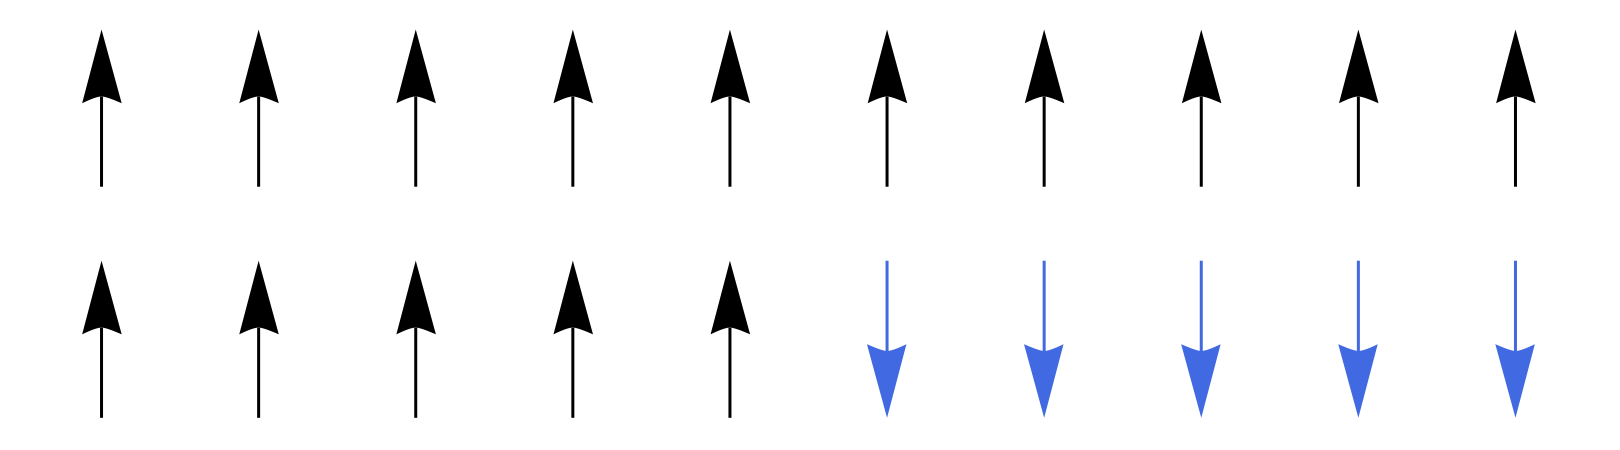
\includegraphics[width=0.8\textwidth]{figures/one-dim-entropy.png}
    \caption{\kaishu 一维 Ising 模型的熵焓竞争}
    \label{fig:一维 Ising 模型的熵焓竞争}
\end{figure}

\textcolor{RoyalBlue}{\textbf{\kaishu 对于周期边界的二维 Ising 链}},一个区域的边界大小是随着区域大小的增加而增加的,所以如果我们将一致向上的 $N$ 个自旋磁子取出一部分磁畴翻转下去,那么相对最初的状态,能量变化 $\delta E \propto N^{1/2}$ 。但由于最多只能有 $N^\alpha$ 种可能的方式达成这一点,那么熵的变化为 $\alpha k\ln N$ 。这个时候,再写出自由能的变化:
\[
    \delta G = \delta E - T\delta S = -N^{1/2} + \alpha kT\ln N
\]
在热力学极限下,第一项就会超过第二项,也就是能量占优,磁畴的翻转变得困难,所以更倾向于保持同向,也就是相变。


\begin{figure}[ht]
    \centering
    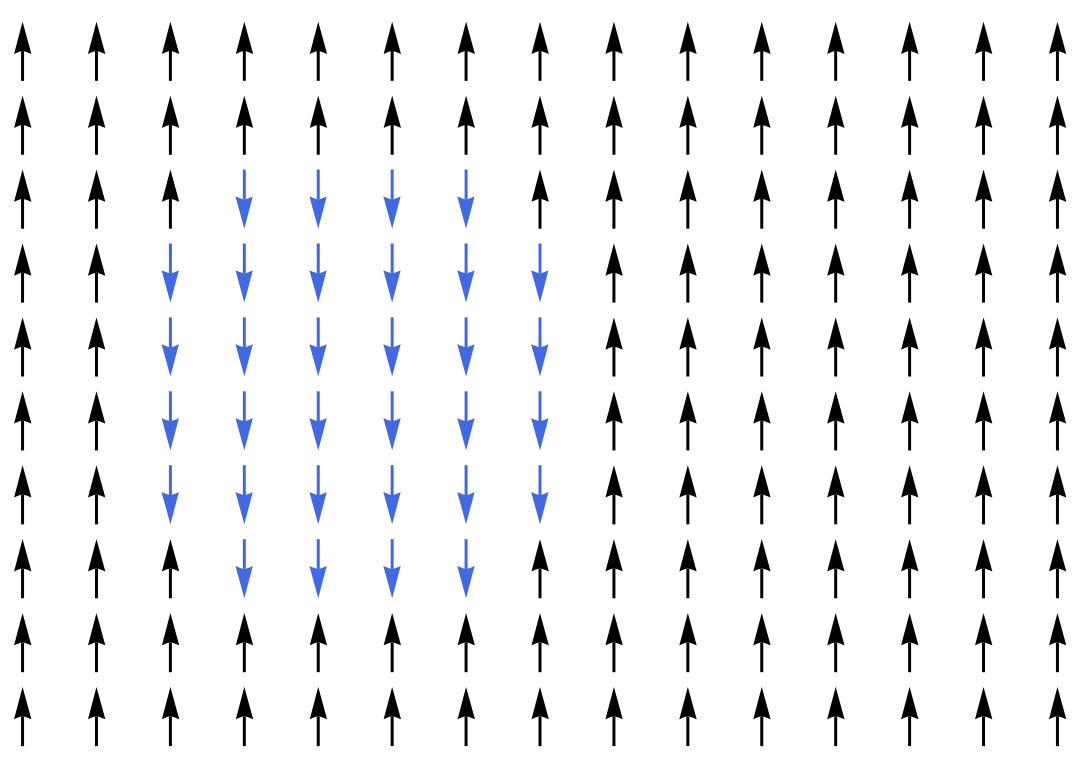
\includegraphics[width=0.7\textwidth]{figures/two-dim-entropy.png}
    \caption{\kaishu 二维 Ising 模型的熵焓竞争}
    \label{fig:二维 Ising 模型的熵焓竞争}
\end{figure}

这也就解释了为什么我们实际观察到体系的对称性要小于系统哈密顿量的对称性,也就是 \textcolor{RoyalBlue}{\textbf{\kaishu 对称破缺}} 的问题。磁学系统哈密顿量虽然具有自旋翻转的对称性(系统所有自旋全部翻转,总能量不变),但要想在实际中体现这一点, \textcolor{RoyalBlue}{\textbf{\kaishu 必须要求这个态要能够自由地变换到另一个对称态。}} 但如前所见,这样的翻转动作将会面临巨大的能垒,且在热力学极限下能垒高度为正无穷,所以动力学上不能发生。用一个公式来表示就是:
\begin{equation}\label{equ:对称性破缺}
    \langle M \rangle  = \lim_{H\rightarrow 0}  \lim_{N\rightarrow \infty} \left(-\frac{\partial G}{\partial H}\right)_T \neq 0  
\end{equation}
\textcolor{RoyalBlue}{\textbf{\kaishu 在 $N$ 有限的情况下,系统可以随意翻越能垒,所以磁矩可以为 $0$ ;现在为系统增加一个外场,那么系统将会聚集在某一边。现在让 $N\rightarrow \infty$ ,把门关上,系统就被困在了一个状态,纵使外场消失,系统即使想回去,也回不去了。所以宏观磁矩不为 $0$ ,这就是对称性破缺的本质。}}

\subsection{一维 Ising 模型的严格解}\label{sub:一维Ising模型的严格解}

下面我们正式进入一维 Ising 模型的严格解。我们先来考虑无外场周期性边界一维 Ising 模型的配分函数:
\begin{equation}\label{equ:一维Ising模型的配分函数}
    Q_N = \sum_{S_1,S_2,S_3,\cdots S_N} \exp\left[K' (S_1 S_{2}+S_2S_3+\cdots+S_NS_1)\right]
\end{equation}
我们将它改写为如下形式:
\begin{equation}
    Q_N = \sum_{S_1,S_2,S_3,\cdots S_N} \exp(K' S_1 S_{2}) \exp(K' S_2 S_{3}) \cdots \exp(K' S_N S_{1})
\end{equation}
这样一来,我们就可以将配分函数视为 \textcolor{RoyalBlue}{\textbf{\kaishu 张量缩并}}。为了看出这一点,将 $\exp(K' S_1 S_2)$ 写成矩阵的形式:
\begin{equation}
    T(S_1,S_2) = \exp(K' S_1 S_{2}) = \begin{pmatrix}
        e^{K'} & e^{-K'} \\
        e^{-K'} & e^{K'}
    \end{pmatrix}
\end{equation}
这叫做 \textcolor{RoyalBlue}{\textbf{\kaishu 转移矩阵}} ,再把被求和的 $\{S_1,S_2,\cdots,S_N\}$ 视为哑标,那么配分函数就可以写成:
\begin{equation}
    Q_N = \sum_{S_1,S_2,S_3,\cdots S_N} T(S_1,S_2) T(S_2,S_3) \cdots T(S_N,S_1) = \text{Tr}(T^N) = \lambda _1^N + \lambda_2^N
\end{equation}
其中 $\lambda_1,\lambda_2$ 是转移矩阵的两个本征值,易得
\begin{equation}
    \lambda_{1,2} = e^{K'} \pm e^{-K'}
\end{equation}
所以配分函数可以写成
\begin{equation}
    Q_N = (2\cosh K')^N + (2\sinh K')^N
\end{equation}

如果有外场,那么我们需要对外场所导致的额外能量做一点变换,因为要想构成二维张量,需要两个自旋:
\[
    E = -\sum_{i=1}^N JS_i S_{i+1} - \mu H\sum_{i=1}^N S_i = -\sum_{i=1}^N JS_i S_{i+1} - \frac{\mu H}{2} \sum_{i=1}^N (S_i + S_{i+1})
\]
其中 $S_{N+1} = S_1$ 。转移矩阵就变成了
\begin{equation}
    T(S_1,S_2) = \exp(\frac{1}{2}K (S_1+S_2) + K' S_1 S_{2}) = \begin{pmatrix}
        e^{K+K'} & e^{-K'} \\
        e^{-K'} & e^{-K+K'}
    \end{pmatrix} 
\end{equation}
本征值
\begin{equation}
    \lambda_\pm = \mathrm{e}^{ K'}\left(\cosh K \pm \sqrt{\sinh ^2 K + \mathrm{e}^{-4 K'}}\right)
\end{equation}
在热力学极限下,较小的特征值 $\lambda_2$ 将会被忽略,所以配分函数可以写成
\begin{equation}
    Q=\mathrm{e}^{N K'}\left(\cosh K+\sqrt{\sinh ^2 K+\mathrm{e}^{-4 K'}}\right)^N
\end{equation}
由此可得磁学系统的各热力学函数:
\begin{align*}
    &G\bigg|_{H=0} = -kT\ln Q = -NkT \ln (e^{\beta J} + e^{-\beta J}), \\
    &S\bigg|_{H=0} = \frac{\partial G}{\partial T} = Nk\left[\ln (e^{\beta J} + e^{-\beta J}) - \beta J \tanh\beta J\right],\\
    &U\bigg|_{H=0} = G + TS =  NJ \tanh\beta J,\\
    &C\bigg|_{H=0} = \frac{\partial U}{\partial T} = Nk\beta^2 J^2 \mathrm{sech}^2 \beta J,\\
    &\langle M \rangle = \frac{\partial \ln Q}{\partial \beta H} = \frac{\mu N\sinh \mu \beta H}{\sqrt{\sinh ^2 \mu \beta H+\mathrm{e}^{-4 \beta J}}},\\
    &\chi = \frac{1}{N} \frac{\partial \langle M \rangle}{\partial \beta H} = \frac{\mu^2 \mathrm{e}^{-4 \beta J}\cosh \mu\beta H}{\left(\sinh ^2 \mu \beta H+\mathrm{e}^{-4 \beta J}\right)^{3/2}}
\end{align*}

在 $\beta \rightarrow 0$ 时,$S \rightarrow Nk\ln 2$ ,表明系统有 $2^N$ 的配容数;在 $\beta \rightarrow \infty$ 时,$S \rightarrow 0$ ,表明系统处于绝对零度。对于响应函数,当 $H \neq 0$ ,温度趋于 $0$ 时收敛为 $0$ ;而当 $H = 0$ ,温度趋于 $0$ 时发散。

\begin{justification}{\kaishu 反思与质疑}
\kaishu \fontsize{11pt}{16pt}
\quad\quad 容易看出,转移矩阵方法其实也可以用在非周期条件上,只不过不再是张量的求和缩并为迹,而是张量的求和缩并为张量。这样一来,我们就可以将一维 Ising 模型的配分函数写成
\begin{equation}
    Q_N = \sum_{S_1,S_2,S_3,\cdots S_N} T(S_1,S_2) T(S_2,S_3) \cdots T(S_{N-1},S_{N}) = \sum_{S_1, S_N} T^{N-1}
\end{equation}
也就是矩阵 $T^{N-1}$ 的所有项之和。

\quad\quad 当然,转移矩阵并不一定是 $2$ 维的,所以如果系统有三个可能状态,$S_i$ 的可能取值为 $1,0,-1$ ,那么无外场转移矩阵为
\begin{equation}
    T = \begin{pmatrix}
        e^{K'} & 1 & e^{-K'} \\
        1 & 1 & 1 \\
        e^{-K'} & 1 & e^{K'}
    \end{pmatrix}
\end{equation}
而实对称阵必能正交相似对角化,所以我们总是可以通过正交相似变换来计算 $T^N$ 的特征值。
\end{justification}

\subsection{二维 Ising 模型概要}\label{sub:二维 Ising 模型概要}

二维 Ising 模型的解析解由杨振宁完成,这里只给出一些基本结果,不做推导。

在 $H = 0$ 的条件下,二维 Ising 模型的配分函数为
\begin{equation}
    Q(N,\beta,0) = \left[2\cosh (2\beta J e^I)\right]^N
\end{equation}
其中
\begin{align*}
    &I = \frac{1}{2\pi} \int_0^\pi \ln \left[\frac{1}{2} \left(1 + \sqrt{1 -K(J)^2\sin^2 \theta}\right)\right] \mathrm{d}\theta, \\
    &K(J) = \frac{2\sinh 2\beta J}{\cosh^2 2\beta J}
\end{align*}
当 $K(J) = 1$ 时,系统可能出现奇异性,也即相变点满足
\begin{equation}
    \sinh 2\beta_c J = 1
\end{equation}
数值结果约为
\begin{equation}
    kT_c \approx 2.269J
\end{equation}
而每个自旋的平均值为
\begin{equation}
    m = \frac{\langle M \rangle}{N} = \left\{\begin{aligned}
        &0 && T > T_c \\
        &\left[1 - \sinh^{-4} 2\beta J\right]^{1/8} && T < T_c
    \end{aligned}\right.
\end{equation}

\section{Ising 模型的零级近似:平均场理论}\label{sec:Ising 模型的零级近似:平均场理论}

Ising 模型的解析解的求解难度随着维数的增加而增加,三维 Ising 模型没有解析解,只能通过数值模拟的方法完成。这表明 Ising 模型本身仍然需要做一定的近似,使得高维 Ising 模型也有近似的解析解。

\textcolor{RoyalBlue}{\textbf{\kaishu 平均场理论}}  就是这样一种近似方法。回想我们在无相互作用系统中的高光时刻,如果我们能将每个 Ising 磁子受到的相互作用以一个等价的平均外场来替代,那么我们就可以将 Ising 模型转化为一个无相互作用的模型,配分函数瞬间就变为了单粒子配分函数的 $N$ 次方。

\subsection{基本结果}\label{sub:基本结果}
现在我们来将单粒子近似用到统计力学里来(Hartree-Fork理论或者金属能带论都有涉及)。既然是平均场,那么自旋势必需要做一点平均:
\begin{equation}
    \langle S_i \rangle = \frac{\langle M \rangle}{N} \equiv m
\end{equation}
这里的 $m$ 有一个特殊的名称: \textcolor{RoyalBlue}{\textbf{\kaishu 序参量}}。将字面意义与物理意义结合起来看,这个量刻画了系统的有序程度。设每个磁子周围都有 $z$ 个其他磁子,那么磁子 $i$ 的能量为
\begin{equation}
    E_i = -\mu HS_i - J \sum_j S_i S_j = -\mu HS_i - zJmS_i
\end{equation}
单粒子配分函数与 $S_i$ 的平均值为
\begin{align}
    Q_1 &= \sum_{S_i = \pm 1} e^{\beta \mu HS_i + \beta zJmS_i} = 2\cosh (\beta \mu H + \beta zJm),\\
    \langle S_i \rangle &= \frac{\partial \ln Q_1}{\partial (\mu\beta H)} = \tanh (\beta \mu H + \beta zJm)
\end{align}
然而,系统的每个磁子都是等价的,所以 $S_i$ 本身的平均值也应当是 $m$。换言之,为了使得我们的理论自洽,必须有如下的 \textcolor{RoyalBlue}{\textbf{\kaishu 自洽场方程}}:
\begin{equation}
    \begin{aligned}
        m &= \tanh (\beta \mu H + \beta zJm)\\
        \beta &= \frac{1}{2zJm} \ln \frac{1+m}{1-m} 
    \end{aligned}
\end{equation}
在外场为 $0$ 的条件下,显然 $m = 0$ 为平凡解。要想得到非平凡解,根据函数的性质,必须要求
\begin{equation}
    \frac{\partial \tanh (\beta zJm)}{\partial m} \bigg|_{m = 0} > 1 \quad \Rightarrow \quad \beta zJ > 1 \quad \Rightarrow \quad T_c = \frac{zJ}{k} = \left\{\begin{aligned}
        &\frac{2J}{k} && \text{one dimention} \\
        &\frac{4J}{k} && \text{two dimention} \\
        &\frac{6J}{k} && \text{three dimention} 
    \end{aligned}\right.
\end{equation}

平均场方程是一个非线性方程,我们可以通过数值方法求解,结果绘制在图 (\ref*{fig:one-dim-ising}) 中:
\begin{figure}[ht]
    \centering
    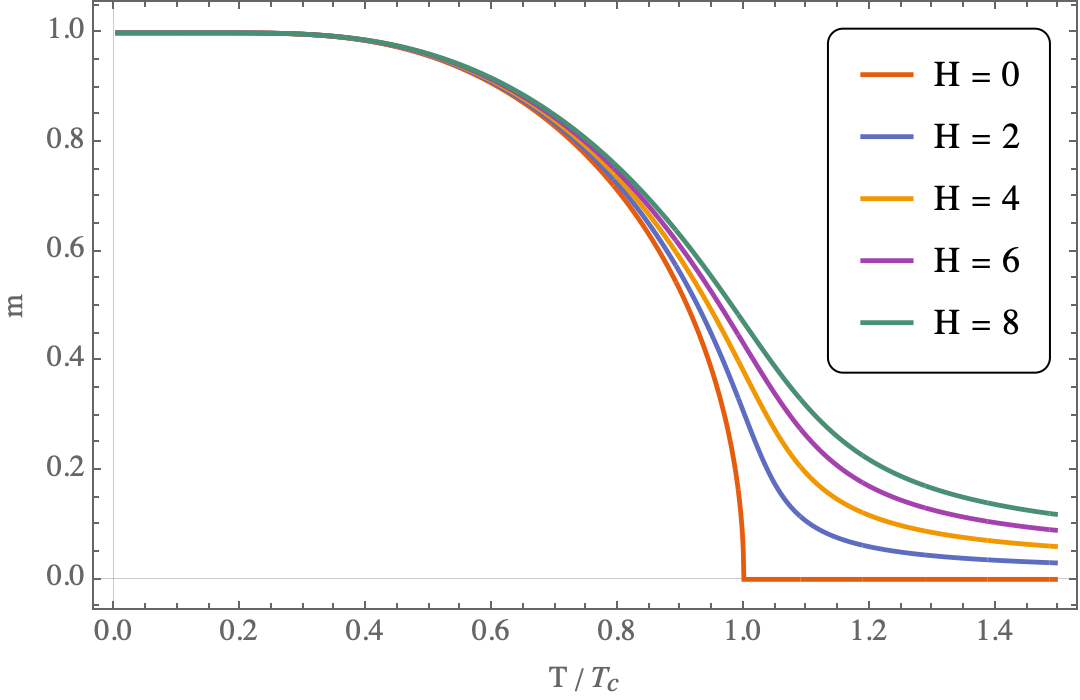
\includegraphics[width=0.7\textwidth]{figures/mean-field-mean-spin.png}
    \caption{\kaishu 平均场序参量随温度的变化情况}
    \label{fig:one-dim-ising}
\end{figure}

\begin{justification}{\kaishu 反思与质疑}
\kaishu \fontsize{11pt}{16pt}
\quad\quad 三维 Ising 模型的临界温度的模拟结果为 $4J/k $ ,可见平均场理论总是高估相变温度。这是因为它仅仅考虑一个磁子在平均场下的涨落,而忽略了其他磁子的涨落——将取向一致的一碗米粒稍微摇晃一下,米在碗中的高度将会继续下降。
\end{justification}

\subsection{临界行为}\label{sub:临界行为}

\begin{figure}[ht]
    \centering
    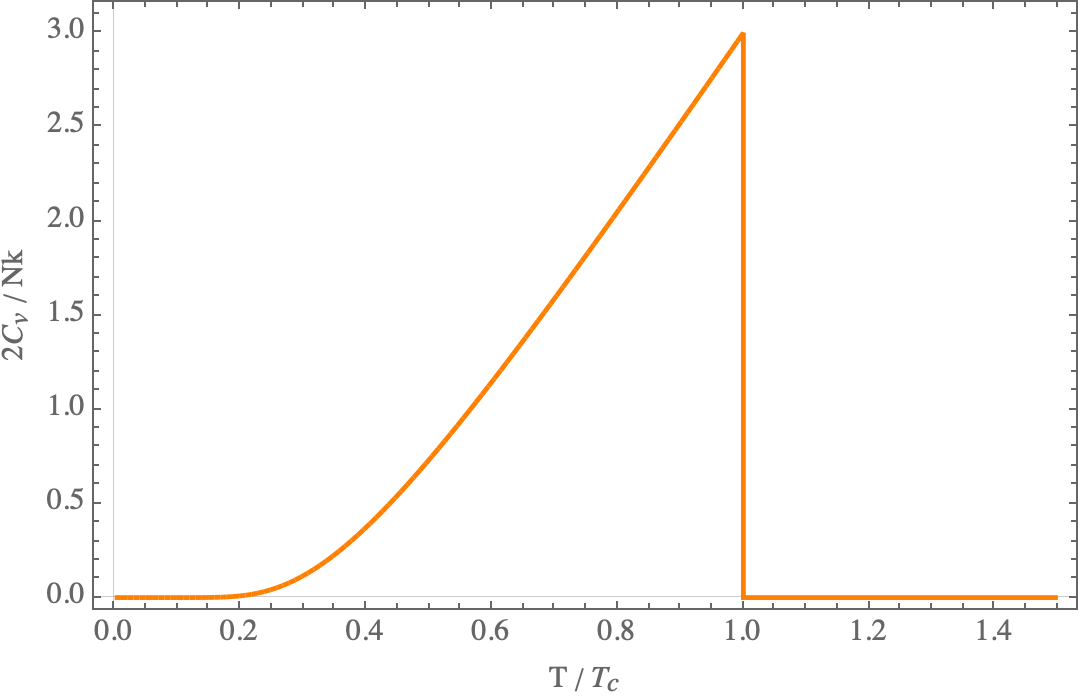
\includegraphics[width=0.7\textwidth]{figures/meanfield-heat-capacity.png}
    \caption{\kaishu 系统热容随温度的变化情况}
    \label{fig:sol-capa}
\end{figure}

\subsection{响应函数与关联函数}\label{sec:响应函数与关联函数}

自旋作为两个随机变量,它们之间的关联性,可以用 \textcolor{RoyalBlue}{\textbf{\kaishu 协方差}} 来描述:
\begin{equation}
    \text{Cov}(S_1,S_2) = \langle S_1 S_2 \rangle - \langle S_1 \rangle \langle S_2 \rangle
\end{equation}
平均场近似认为各自旋变量都是独立的,所以自然有 $\text{Cov}(S_1,S_2) = 0$ 。下面我们来讨论响应函数和关联函数之间的联系,只需指出:
\begin{equation}
    \begin{aligned}
        \chi &= \frac{1}{N} \langle (M-\langle M \rangle)^2 \rangle \\
        &= \frac{\mu^2}{N}\langle \left[\sum_i^N S_i - \langle S_i \rangle\sum_j^N S_j - \langle S_j \rangle\right] \rangle \\
        &= \frac{\mu^2}{N} \sum_{i,j}\text{Cov}(S_i,S_j) = \mu^2 \sum_{j}^N\text{Cov}(S_1,S_j)
    \end{aligned}
\end{equation}
那么响应函数是关联函数的总和,响应函数要想发散,各处的关联函数必须全都大于 $0$ ,这也表明关联尺度发散。


\subsection{平均场的变分方法}\label{sub:平均场的变分方法}


\section{重正化理论}

\textcolor{RoyalBlue}{\textbf{\kaishu 响应函数 $\chi$ 的发散究竟反映了什么物理?}}

“系统本身的涨落越大,那么对外界的响应就越灵敏”这句话,实际上蕴含了这样一则惊天秘闻:系统对外界的响应是一种宏观性质,当整个系统都“合作起来”对外界变化产生响应时,意味着能参与合作的范围,也就是 \textcolor{RoyalBlue}{\textbf{\kaishu 关联尺度}},开始发散。一个例子便是液体的临界乳光现象,透明的水在临界点附近变为乳白色,这表明本应当从水分子的间隙中漏过大部分的自然光,却大部分被散射了。这样的现象只有一种解释:水分子不再是孤立的,而是形成了一个个的团簇,这些团簇的尺度越来越大,最后甚至大到与光的波长相当,从而产生了散射——把渔网加密,就能捞到更小的鱼。

那么问题来了:如果水分子的关联尺度发散,那么多少水分子能算一个团簇?这相当于询问临界水的 \textcolor{RoyalBlue}{\textbf{\kaishu 特征尺度}} 是多少。仔细想想,我们发现这个问题无法回答,因为关联尺度发散意味着一个水分子和无穷远的另一个水分子都有相互作用,这个特征尺度是不存在的。

特征尺度一旦不存在,我们发现系统将会呈现出 \textcolor{RoyalBlue}{\textbf{\kaishu 自相似}} 的特征(例如分形),这也是相变非常典型的特征:用不同尺度的放大镜来观察相变,得到的结果都是相似的。

这样一来,在相变点附近,多自由度系统能够合理合法地约化到低自由度系统,并且相变点系统的形貌在 \textcolor{RoyalBlue}{\textbf{\kaishu 尺度变换}} 下不变。

也就是说: \textcolor{RoyalBlue}{\textbf{\kaishu 相变点是尺度变换的不动点。}}

\subsection{卡丹诺夫变换}

这一节写一维伊辛模型,分为无外场和有外场,指出一维没有相变。

\subsection{二维 Ising 模型的重正化}

抄chandeler 的书

\section{总结}